
\newpage

\section{Classification based techniques}

Classification based techniques are based on systematic learning approaches based on sets of data. 
The supervised approaches requires knowledge to train a model (or classifier) from a set of data instances (or training data) and classifies a new data instance as normal or as outlier. 
The unsupervised approaches do not require knowledge and learn the boundary around normal instances, declaring the new instance as normal or as outlier depending if the data instance is outside of the boundary of the previous data sets.

The classification based techniques are listed as the following:

\begin{itemize}
	\setlength\itemsep{-0.5em}
	\item Neural Networks-based;
	\item Bayesian Networks-based;
	\item Rule-based;
	\item Support Vector Machines-based.
	
\end{itemize}

Neural networks-based approaches are interesting strategies for outlier detection where a given neural network might be trained with only normal data-sets. 
At testing stage, the data instances that are similar to the training data-set are accepted by the neural network and then considered as normal. 
The remaining data-sets are rejected by the neural network due to their lack of similarity with normal data-sets. Thus, those data instances are considered as outliers. 
Based on the table \ref{table:t3}, these techniques are classified as semi-supervised due to their need for normal data-sets for the training stage.

Bayesian networks-based approaches are identified as prominent techniques for outlier detection in WSNs, being the reason why they are extensively covered further on.
Those techniques ...

Rule based ...

Support Vector Machine (SVM) relies on ...

\subsection{Bayesian Networks}

Zhang et al. <zhang2010> divide the bayesian network based techniques in three categories: 

\begin{itemize}
	\setlength\itemsep{-0.5em}
	\item Na\"{i}ve Bayesian Networks;
	\item Bayesian Belief Networks;
	\item Dynamic Bayesian Network Models;	
\end{itemize}

All those approaches uses probabilistic graphical models to represent a set of variables and their probabilistic interdependencies. 
This graphical model aggregates the information from different variables and provides an estimate on the expectancy of an event to belong to the learned class.

Xiang et al. <xiang2015> illustrates an application to measure the concentration of NO$_2$, CO and O$_3$ pollutants, using a bayesian network. All the three variables are all correlated and also depends on the temperature as presented in figure \ref{fig:xiang2016}. The real measurements acquired by the microcontroller are represented with (s) and the representations in (t) refers to the real concentration of those pollutants.

\begin{figure}[h!]
	\centering
	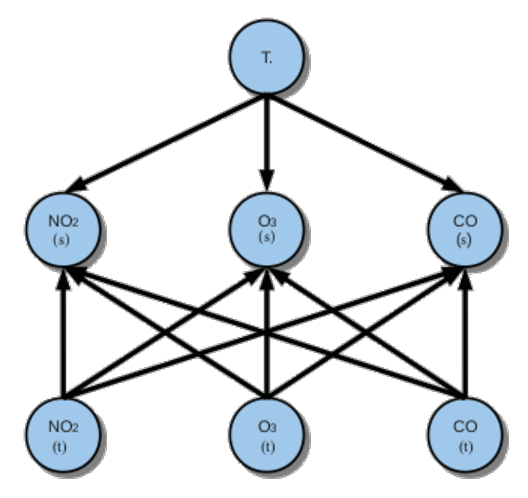
\includegraphics[width=0.60\textwidth,keepaspectratio]{figures/xiang2016}
	\caption{Application of a Bayesian Network to an atmospheric measurement system. }
	\label{fig:xiang2016}
\end{figure}

The three categories presented by Zhang et al. differs between them where the first category captures the sensor nodes correlations on spatio-temporal domain; 
The second one considers not only the spatio-temporal correlations but also the conditional dependence of sensor attributes;
The third category proposes the measurement of state variables at a current time instance.

Janakiram et al. <janakiram2006> proposes the detection of outliers in sensor streamed data by capturing the conditional dependencies among the observation of it's attributes. this is made in three phases:

\begin{description}
	\setlength\itemsep{-0.5em}
	\item[Training Phase]  
	Phase where the Bayesian Belief Network is trained to capture the spatio-temporal correlations.
	\item[Testing Phase]  
	Phase where the trained BBN is tested on the level of accuracy and, if needed, the learned parameters are updated.
	\item[Inference Phase] 
	Phase where the missing values are inferred and the remaining streamed data are tested to detect if it is an outlier or not.
\end{description}

Janakiram et al. also defined the BBN, where the BBN is a directed graph, together with an associated set of probabilistic tables.
The graph is divided in nodes and arcs, where the nodes represents the variables and the arcs are the representation of the casual/influential relationship among variables.

The main contribution of BBN is the possibility to have a model that, with the dependency between uncertain variables (by filling a node probability table), it is possible to describe complex probabilistic reasoning about uncertainty.

Janakriam et al. describes their process in three steps:

\begin{itemize}
	%\setlength\itemsep{-0.5em}
	
	\item Constructing the Bayesian Belief Network
	\subitem \textbf{IF} a few variables have direct dependencies
	\subitem \textbf{AND} many of the variables are conditionaly independent
	\subitem \textbf{THEN} all the probabilities can be computed from the joint probability distribution.
	
	\item Learning Bayesian Belief Networks
	\subitem \textbf{IF} the network structure is given
	\subitem \textbf{AND} all variables are fully observable in the training examples
	\subitem \textbf{THEN} estimating the conditional probabilities is enough
	\subitem
	\subitem \textbf{IF} the network structure is given
	\subitem \textbf{AND} some of the variables are observable
	\subitem \textbf{THEN} apply neural network using Gradient Ascent Procedure
	\subitem
	\subitem \textbf{IF} the network structure is unknown
	\subitem \textbf{THEN} Use heuristic search
	\subitem \textbf{OR} Use constraint-based technique to search through potential structures
	
	
	\item Inferring from Bayesian Belief Networks
	\subitem \textbf{THESIS} The probability distribution of certain attributes might be inferred
	\subitem \textbf{PROOF} Given the fact that the values that other attributes can take are known	
\end{itemize}

Paola et al <paola2014> proposes an adaptive distributed Bayesian approach for detecting outliers in data collected by a WSN.
The focus of the proposed algorithm is the optimization of outlier classification accuracy, time and communication complexity and also considering externally imposed constraints on conflicting goals. The proposed algorithm is intended to run in each sensor node. 

From the individual sensor node point of view, this algorithm consists in two phases:

\begin{description}
	\setlength\itemsep{-0.5em}
	\item[Outlier detection]  
	Where, based on sensor readings and on the collaboration with neighbors, is made the probabilistic inference where the results are evaluated in three metrics: classification accuracy, time complexity and communication complexity.
	
	\item[Neighborhood selection] 
	Where the best neighbors are identified ad selected to cooperate with, and, in addiction, to correspond to a reconfiguration of the Bayesian Network structure.
\end{description}

In the global point of view, if there is a high number of cooperating nodes, the classification is natirally higher with the drawback if increasing the processing time and communication complexity (thus resulting in increased detection delay and increase of energy consumption).

Xiang et al. <xiang2016> proposes the addition of recover and recalibrate the drifted sensors simultaneously based on the usage of a Bayesian network.

The authors have applied their algorithm to the measurement of the variables in the sensor readings of the NO$_2$, CO and O$_3$ pollutants, as previously presented in figure \ref{fig:xiang2016}.
Based on the correlations of the sensor readings and on the temperature influence, the algorithm itself detects the outliers, recover valid information and adjust the BBN to automatically recalibrate the sensor.

\newpage


\subsection{Rule-based techniques}
\lipsum[1]

\subsection{Support Vector Machines}